\graphicspath{{chapters/simulation/images/}}
\chapter{Simulation of the IceCube-DeepCore Detector}
\label{chapter:simulation}
In order to model both signal and background, \emph{Monte Carlo simulations} of the detector are necessary. 
In the search for tau neutrinos, this is particularly important due to the low rates and high backgrounds expected, requiring multiple types of simulation for both signal and background.

Simulation in IceCube is broken into three broad stages, each of which will be discussed in turn.
The generators used in the appearance analysis are discussed in Section~\ref{sec:generators}.
The propagation of the charged leptons and photons are then described in Section~\ref{sec:propagation}.
Section~\ref{sec:electronics} describes the simulation of the detector, including the PMT electronics and the detector noise.

\section{Monte Carlo Generators}
\label{sec:generators}

\subsection{Background Generation}
\label{subsec:bg_generation}

\subsubsection{CORSIKA}
\label{subsubsec:corsika}
The primary background for the observation of atmospheric neutrino events is the other particles present in the cosmic ray interactions in the atmosphere.
These interactions produce many particles, most of which are stopped before reaching IceCube by the shielding provided by the Antarctic Glacier.
In order to correctly account for the interactions and decays of these particles, the \emph{CORSIKA} generator from Karlsruhe Institute of Technology is used \cite{CORSIKA}. 

The CORSIKA generator is a collection of code designed to simulate, interact, and propagate a cosmic ray air shower from the interaction point in the upper atmosphere to a user-defined height. 
Originally designed for use with surface detectors such as Auger, HAWC, and IceTop, the code has been adapted for use in the IceCube collaboration by identifying the muon (and, sometimes, neutrino) components of the air shower.

CORSIKA has many modes of operation and options for configuration. 
The standard IceCube simulation of air showers uses the SIBYLL 2.1 hadronization mode \cite{SIBYLL-2.1} to follow the interactions through the shower. 

IceCube simulation of air showers uses two cosmic ray production modes of CORSIKA: the Polygonato and 5-Component modes.

The "Polygonato" mode generates cosmic rays following the model from \cite{Hoerandel-Polygonato}. 
The Polygonato flux parametrized the energy spectra of individual elements of the cosmic ray flux as power laws extrapolated to high energies.
In typical IceCube simulation, CORSIKA simulation produced using the Polygonato mode includes a mixture of muons from all seasons, effectively producing an averaged flux useful under the assumption of equal livetime throughout the year.
The elemental ratios of the generated cosmic ray primaries follow the Polygonato flux directly, producing a "natural" flux of simulated events \cite{CORSIKA}.
The natural spectrum of the Polygonato CORSIKA simulation has the benefit of allowing a direct physical interpretation of the resulting spectrum without the need for reweighting and simplifies the prodution of coincident showers, which require a natural spectrum.

The second model, the five-component mode, reduces the full spectrum of cosmic rays to five effective families: hydrogen, helium, nickel, aluminum, and iron. 
Each of these components is allowed to have a separate normalization and spectral index.
The five-component mode is useful due to the ease with which the user can modify and reweight to different primary spectra, allowing the investigation of different cosmic ray compositions without the production of dedicated simulation.
The simplicity associated with the reweighting of five-component simulation allows IceCube to produce unphysical spectra in order to optimize the production of simulated events necessary for the various analyses.
The five-component simulation may be reweighted to match cosmic ray models, including both the Polygonato model and the newer H3a model, which models the cosmic ray flux using three distinct populations of sources \cite{Gaisser-H4a}.
While this slightly complicates the use of the simulation in analyses, the ability to evaluate the uncertainties in various cosmic ray models has been an invaluable tool for high energy analyses, which can be sensitive to changes in the cosmic ray spectrum above the knee.

About 10\% of the muons from cosmic ray air showers which reach the IceCube detector will arive temporally coincident with muons from other showers.
Five-component CORSIKA simulation, due to the unphysical generation spectrum, cannot easily be used in the production of these \emph{coincident} events and are currently supplemented by the Polygonato CORSIKA for this purpose.

In both cases, the particles from the air shower are only propagated to the surface of the ice. 
For analyses using the in-ice array, we take the muons reaching the surface from a CORSIKA simulation and propagate them through the ice, simulating the continuous and stochastic energy losses along the way. 
The muons are propagated to a surface in the ice consisting of a cylinder with radius 800 meters and length 1600 m centered on the IceCube detector.
In order to reach the detector, a muon must result from a cosmic ray interaction of approximately 600 GeV due to the shielding of the glacier.
Because of this, CORSIKA simulations typically have a lower energy cutoff of about this value to avoid simulating events that will not reach the detector.

In principle, neutrinos may also be produced using the CORSIKA generator. 
In practice, this tends to be extremely inefficient for most searches that are not explicitly looking for muons and neutrinos from the same air showers given the extremely low cross section of the neutrino relative to the muon.
For this reason, the background generation with CORSIKA in IceCube typically refers to muon events only, with no accompanying neutrino.

\subsubsection{MuonGun}
\label{subsubsec:muongun}
CORSIKA simulations are computationally costly and offer few ways to directly control the spectrum of events at the detector.
Targeted simulations in which particular muon samples are required cannot easily be generated with CORSIKA.
In situations where the required muon simulation falls within a relatively narrow phase space, whether that be in energy, angle, or position inside of the detector, it can be beneficial to tailor simulation to the needs of specific analyses.
Alternatively, there are situations in which the details of the cosmic ray interactions are an unnecessary complication to the final level IceCube analyses.
In these situations, IceCube has developed a tool to bypass the full air shower simulation provided by CORSIKA, producing muons directly at a cylindrical surface inside the ice \cite{Thesis-Jakob}.
This tool, known as \emph{MuonGun}, has the benefit of removing the computationally costly simulation of the full air shower, giving the user more control over the resulting simulated events at the cost of information about the initial cosmic ray interactions.
This allows targeted, high statistics background simulation samples to be produced for analyses.

These features of MuonGun give the generator significant flexibility, allowing for a very focused simulation of muons that would not otherwise be possible with the current implimentation of the CORSIKA generator.
As with all targeted generation, there are limitations to the generation scheme.
For example, the settings described above will provide a good description of muons reaching and triggering the DeepCore array, but will not include the correct contributions of muons in the outer IceCube detector.
This can result in disagreement between data and simulation if the limitations are not acknowledged and accounted for.

This abstraction disassociates the muon at the detector from the air shower, and therefore the cosmic ray, that produced it.
In order to properly account for the dependence on the cosmic ray spectrum in the muon weights, dedicated simulations must be produced using the full CORSIKA generator. 
By following the interaction, showering, and propagation to the detector, IceCube is able to produce an effective parametrization of the association between a particular cosmic ray spectrum and the muons reaching the detector.
This must only be done once, but requires a substantial number of simulated events in order to produce a clean parametrization in position, energy, zenith angle, and variables associated with shower multiplicities higher than one.
The version of MuonGun at the time of writing provides the parametrizations for the Polygonato \cite{Hoerandel-Polygonato} and H4a \cite{Gaisser-H4a} cosmic ray spectra. 
At the time of production for the analyses contained hereafter, all MuonGun simulation is produced assuming a multiplicity of 1, meaning that no bundles are yet produced with this generator.
This is a limitation of simulation time: the multiplicity parametrizations vastly extend the parameter space and therefore require significantly more time and effort to handle correctly.

\subsubsection{Accidental Events}
\label{subsubsec:noise_triggers}
While we only observe Cherenkov photons from neutrino and muon interactions in the detector, we also observe a significant component of \emph{accidental triggers} in the DeepCore array.
These events, produced by detector noise in the detector, result in about 40 Hz of triggered events in IceCube, primarily in DeepCore due to the low trigger threshold.
In these events, no actual particle interactions due to muons or neutrinos are observed.
Instead, detector noise alone satisfies the trigger conditions, producing an event.

Production of accidental triggers involves only the noise and electronics simulation.
Because the events occur as a result of random HLC launches in the detector, the simluation requires a special mode, here called \emph{long-frame} simulation, which produces continuous detector readout. 
Breaking the traditional concept of the "simulated event", these simulation sets instead produce a 100 ms long "event" of random detector noise. 
The photoelectrons from the noise simulation are then run through the simulation of PMT and DOM electronics and triggered as a normal simulated event.
After triggering, specialized code is used to divide the long-frame simulation into smaller events similar to standard IceCube experimental readout.

Once the events are generated, weighting the events is relatively straightforward: the weight per event depends on the muon interaction rate and the total simulated time.
The latter is straightforward to calculate, depending only on the number of long frame simulation events produced and the time window for each of these events.
The former is important due to the definition of the accidental triggers. 
These events, by definition, may only occur when no muon or neutrino is interacting within the detector. 
The weight of the accidental triggers must account for this "deadtime" due to particle interactions.
This particle interaction rate in IceCube is dominated by muons with a rate of approximately 2800 Hz, leading to a change in the effective livetime per accidental triggered event of roughly 15\%..

Accidental triggers are computationally expensive to produce, given that they rely on a relatively rare property of random detector noise. 
The production of accidental triggers takes about one hour per minute of simulated livetime, with much of the processing time spent on the simulation of DOMs that do not contribute to final triggered events.
This limits the total effective livetime that can be simulated in realistic timescales.
Current simulations used in this thesis total approximately two months of effective livetime.

\subsection{Signal Generation}
\label{subsec:signal_generation}

\subsubsection{GENIE}
\label{subsubsec:genie}
Background simulation is only part of the Monte Carlo events in IceCube. 
Studies searching for neutrino candidate events require simulated neutrino signal events to infer properties of the original events.

At energies ranging from approximately 1 GeV to 1 TeV, IceCube has adopted the \emph{GENIE} event generator \cite{GENIE}.
This code, used widely throughout the oscillation community, includes information about the various interactions, cross sections, and uncertainties involved in neutrino physics from reactor energies upward.

For IceCube, events in the GENIE generator are produced from a power law energy spectrum with a given spectral index.
These events are then forced to interact with an electron or nucleon within a specified volume with a target density of ice assumed.

The type of interaction is determined using the cross section for the given flavor and energy.
The cross section model, an updated version of GRV98 \cite{GRV98}, includes resonant, elastic, quasielastic, and deep inelastic interactions.
Particles produced in the interaction are propagated out of the nucleus.
GENIE includes final state interactions where hadrons produced in neutrino interaction can reinteract before escaping the nucleus.
Hadrons with energies less than 30 GeV produced in GENIE simulation are propagated individually to obtain the light output using GEANT4 \cite{GEANT4-1,GEANT4-2}.
Above 30 GeV, the lower event-to-event variability permits the use of parametrized light output for hadrons.
GEANT4 is also used to propagate all muons and tau leptons as well as electrons and photons below 100 MeV.

The GENIE code includes tools to reweight events based on uncertainties in eg. the axial masses, cross sections, and various aspects of the interactions themselves \cite{GENIE}. 
These features are used to model uncertainties in the tau neutrino analysis presented in this thesis.

The code is regularly updated, including both new features and retuning of parametrizations to match the latest data.
The events produced in this work use GENIE version 2.8.6.

\subsubsection{Neutrino-Generator}
\label{subsubsec:nugen}
At energies higher than approximately 100 GeV, there are two changes to the simulation code.
At these energies, the contribution to the cross section from deep inelastic interactions becomes dominant while the other interactions become negligible, as expected from Figure~\ref{fig:xsec} \cite{Formaggio-Xsec}. 
This allows the simplication of the cross section calculations with no loss in generality.
In addition, the cross section continues to rise approximately linearly with the energy.
This latter feature requires a detailed simulation of potential interactions far from the detector: namely, high energy neutrinos have a non-negligible chance of interacting while propagating through the Earth.

The \emph{Neutrino-Generator} code (hereafter, \emph{NuGen}) is designed to handle these higher energy interactions \cite{NuGen}.
In this model, neutrinos are no longer produced and forced to interact in the ice directly.
Instead, a neutrino is produced from a power law spectrum in the atmosphere surrounding the Earth.
The event is then propagated through the planet, using the PREM model of the density layers in the Earth \cite{PREM} to simulate potential interactions en route. 
Neutrinos which interact may be lost or may be regenerated following the decay of the daughter particles.
Neutrinos arriving at the detector are then forced to interact in the detector fiducial volume, yielding a simulated event.

NuGen can be configured with various Earth models as well as different generation properties. 
For the studies contained herein, the NuGen files are produced with an $E^{-2}$ spectrum and interact following the CSMS cross section \cite{CSMS}.












\section{Propagation of the Particles and Light}
\label{sec:propagation}
After production of simulated particle interactions, IceCube simulated events require two types of \emph{propagation}.
The first, the propagation of charged leptons and individual hadrons below 30 GeV, produces the energy losses in the detector due to continuous and stochastic emissions.
These energy losses are then used to produce photons that are propagated through the detector using models of the Antarctic glacier.


\subsection{Lepton Propagation with PROPOSAL}
\label{subsec:proposal}

\begin{figure}
\centering
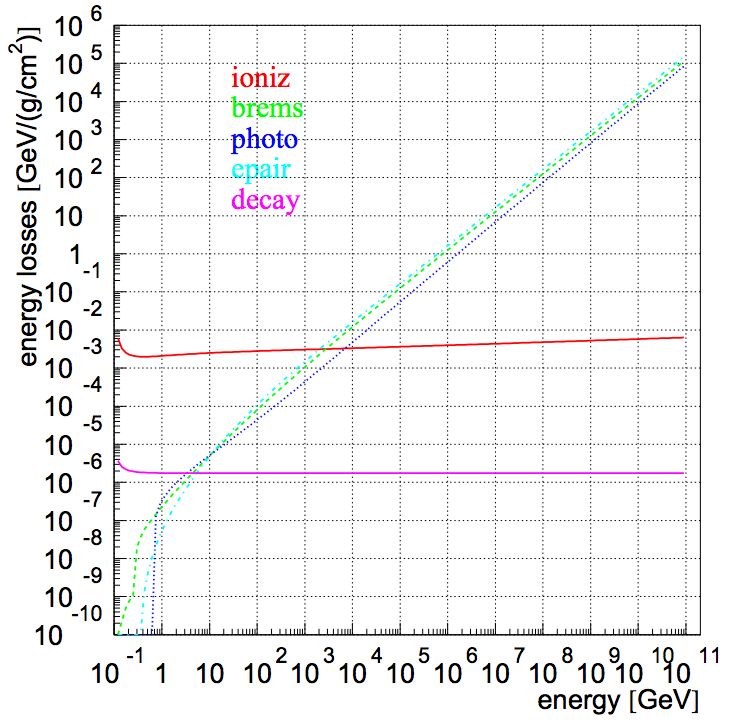
\includegraphics[width=0.6\linewidth]{discrete_emissions_MMC.png}
\caption[Energy losses for a muon in ice]{Average energy losses ($\mathtt{\frac{-dE}{dX}}$) for a muon in ice. At very low energies, ionization losses dominate. Above approximately 1 TeV, pair production and photonuclear effects become more important. Image taken from \cite{Dima-MMC}}
\label{fig:discrete_emissions}
\end{figure}

In IceCube, leptons and hadrons not propagated using GEANT4 are propagated by \emph{PROPOSAL}, a software package containing parametrizations of the ionization, electron pair-production, bremsstrahlung, photonuclear interactions, and decay processes of particles in ice \cite{PROPOSAL}.

PROPOSAL propagates the charged particles through the detector, simulating these processes to give energy emissions along the path of each particle.
The eenergy losses of particles  in the ice is handled by parametrizations as a function of particle energy as shown in Figure~\ref{fig:discrete_emissions}.


\subsection{CLSim for Photon Propagation}
\label{subsec:clsim}
Once the energy deposition for each particle simulated with GEANT4 and PROPOSAL, the resulting photons must be produced and propagated. 
There exist two modules which can handle this: Photon Propagation Code \emph{PPC} and OpenCL Simulation Code \emph{CLSim}. 
The differences are largely of implementation details and both have been verified to give identical results.
Only the latter, CLSim, will be discussed here.

CLSim is a code designed to propagate emitted photons using ray tracing algorithms \cite{PPC}.
The independence of the individual photons is leveraged to perform the propagation of all photons in parallelized calculations using the OpenCL programming language \cite{OpenCL}.
Photons are then propagated through the ice with the model of the scattering and absorption properties, continuing until they are either absorbed or until they reach a DOM.
Photons which reach DOMs are stored to be used in the simulation of the IceCube PMTs.

The propagation of individual photons is efficient at low energies, where the scattering of individual photons is important.
At energies above a few hundred GeV, the light yield is large enough that the propagation of individual photons is both excessively costly as well as unnecessary.
In those cases, a feature known as \emph{oversizing} is used by setting a \emph{oversize factor}, $N_{OS}$.
The oversize factor, often set to 5 for IceCube simulations above 1 TeV, allows for the production of \emph{weighted photons}.
These weighted photons each represent $N^2_{OS}$ individual photons, reducing the number of particles to propagate by $1/N^2_{OS}$.
In order to compensate for the bundling of photons, the effective radius of the DOM is also increased by $N_{OS}$.

Oversizing is efficient for the simulation of high energy events with large numbers of photon.
This breaks down at GeV energies, where the photon flux from an event is low and scattering or absorption of individual photons matters.
Because of the complications associated with oversizing at low energies, most simulations of DeepCore events are done with the oversizing features disabled.

\subsection{Angular Acceptance and Hole Ice}
\label{subsec:holeice_sim}

\begin{figure}
\centering
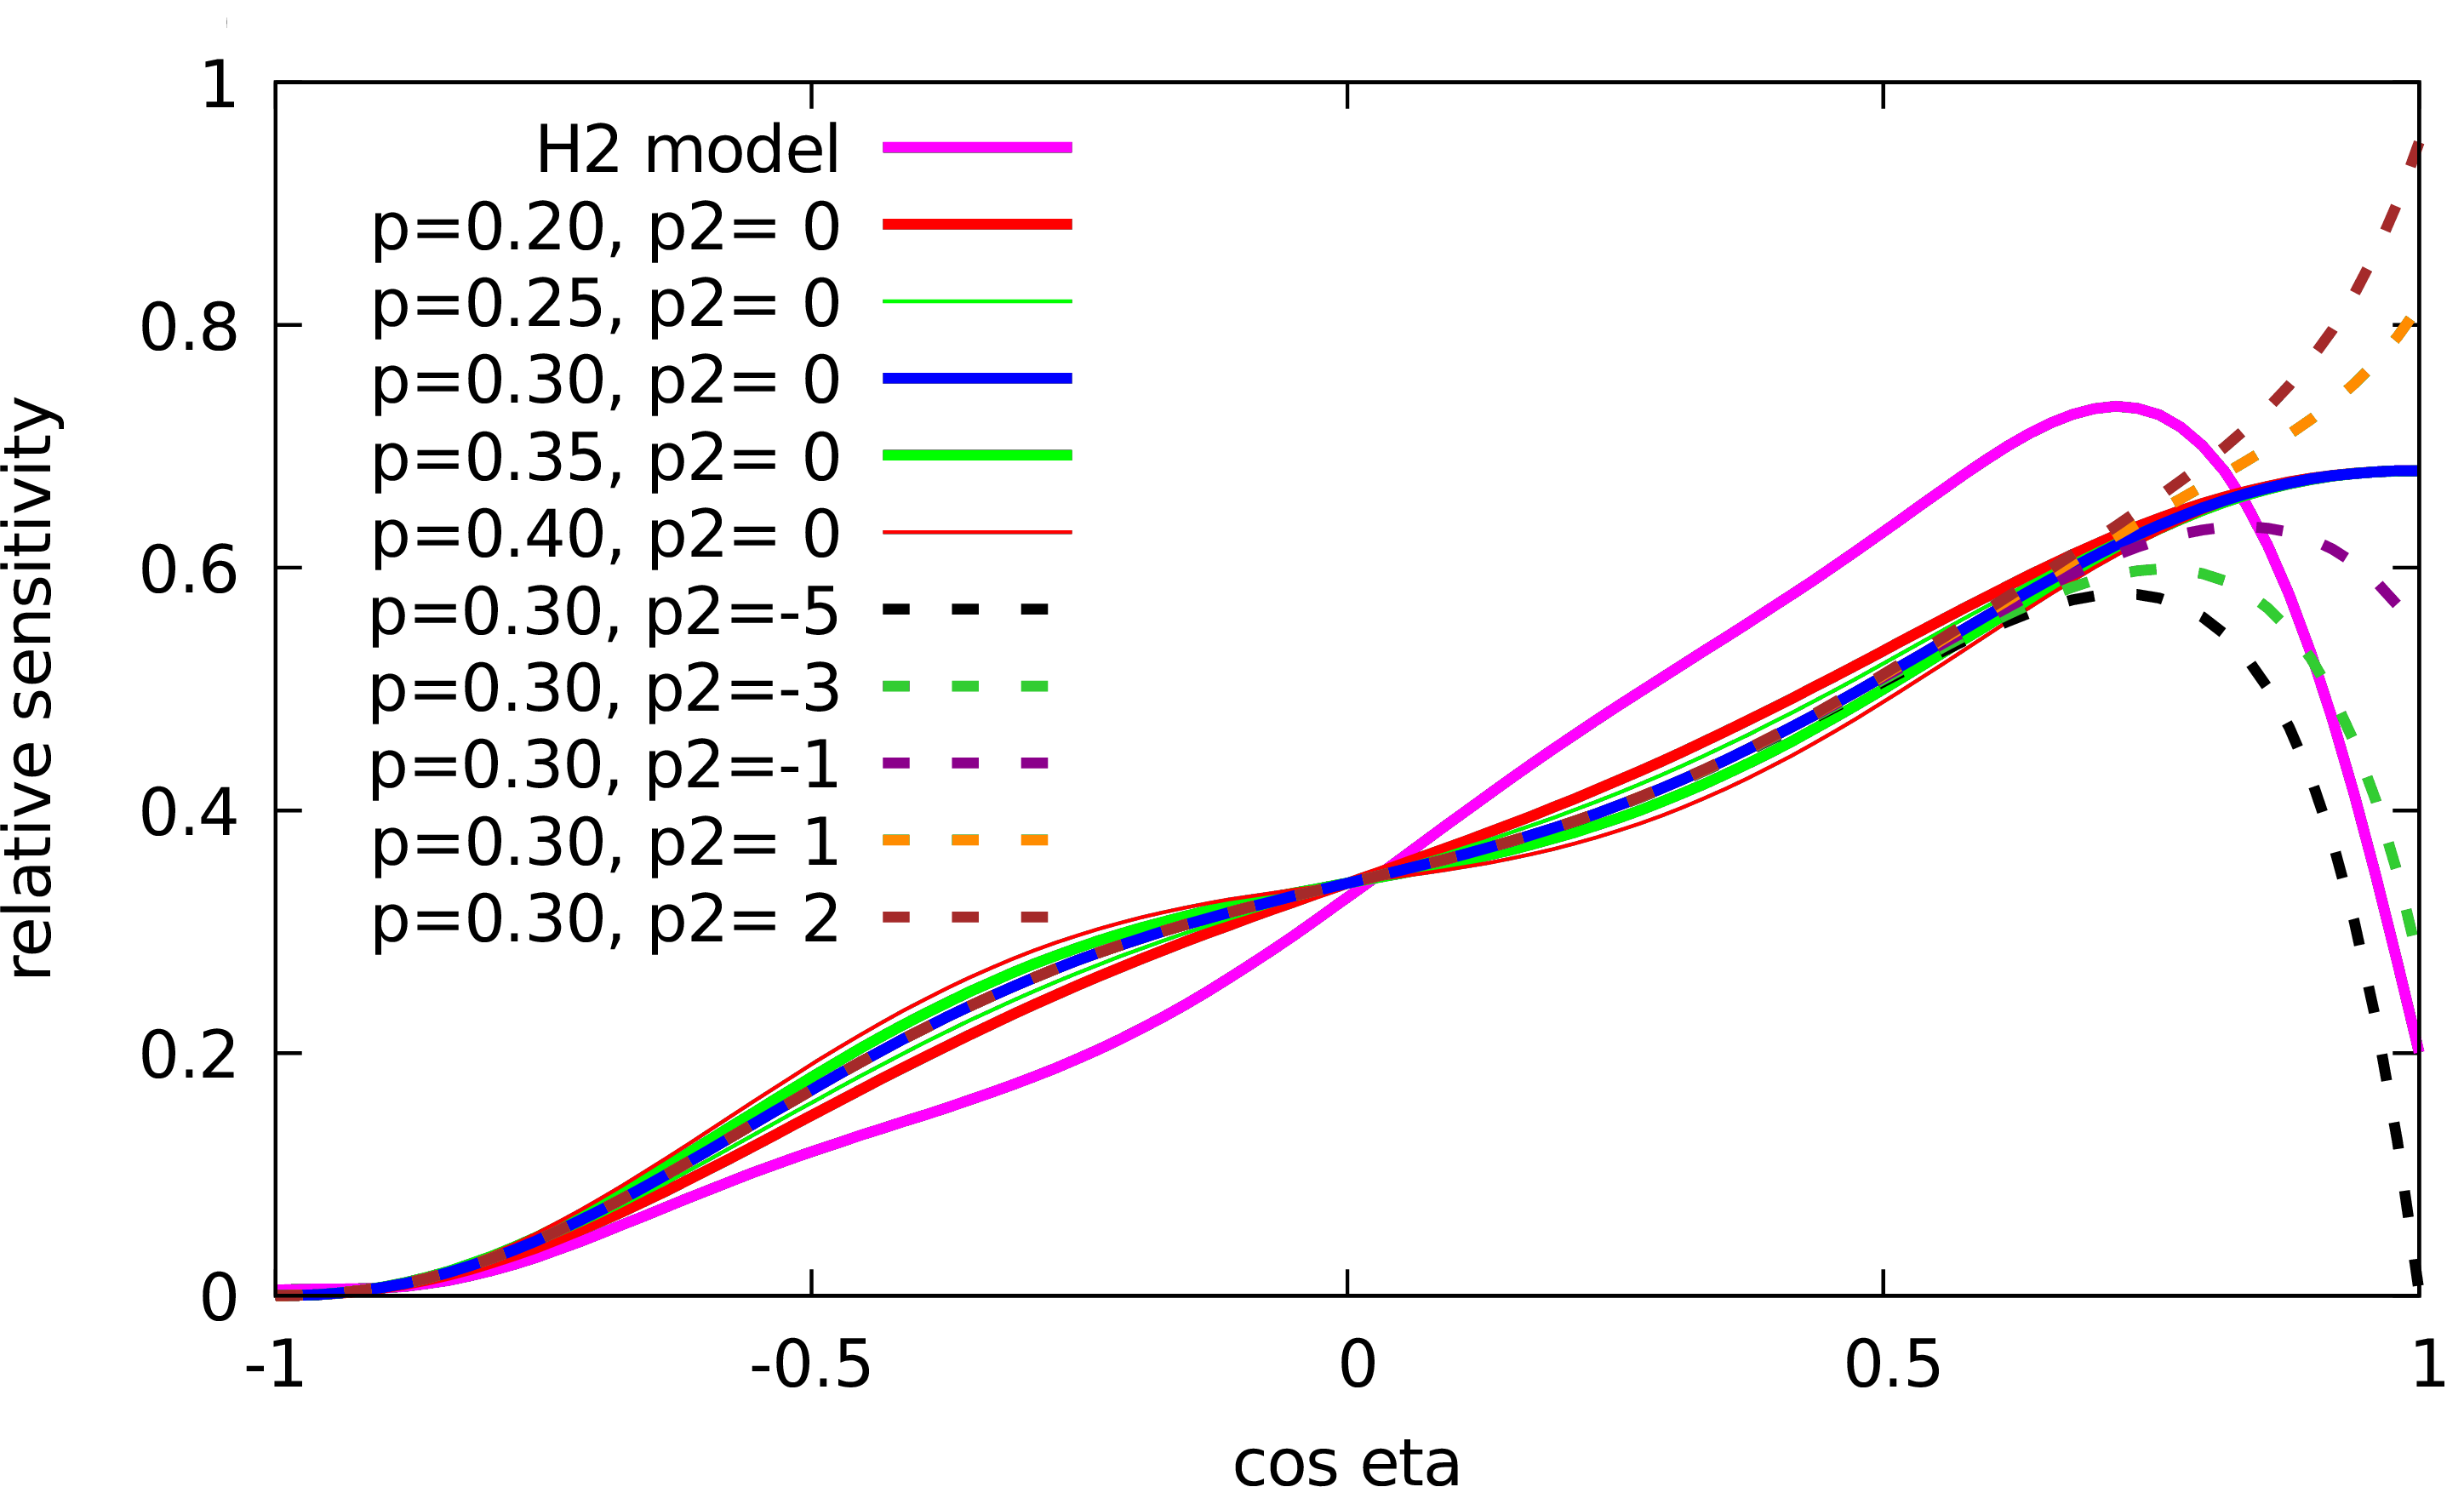
\includegraphics[width=0.7\textwidth]{angular_acceptance.png} 
\caption[Angular acceptance models for IceCube hole ice]{Examples of the angular acceptance models used by IceCube. The relative sensitivity as a function of arrival direction is shown with cos(eta)=-1 indicating the back of the PMT and cos(eta)=1 the face. The variation of the acceptance model used for this search is shown by varying two parameters in the model. The 'p' parameter primarily controls the acceptance at the side of the DOM while the 'p2' parameter controls the acceptance from the forward region. A second model, H2, is also shown.}
\label{fig:angular_acceptance}
\end{figure}

When photons reach the surface of a DOM, the \emph{angular acceptance} is applied in order to model the impact of the hole ice.
This acceptance, calculated from a combination of lab and in-situ measurements, represents the PMT efficiency as a function of the photon arrival direction.
The acceptance has a negligible efficiency for photons arriving from the back of the PMT and higher efficiency for photons reaching the face of the PMT as shown in Figure~\ref{fig:angular_acceptance}.
All other directions follow a curve between these two points.
The angular acceptance model used in this thesis uses an empirical form fit to flasher data with two free parameters, as shown in Figure~\ref{fig:angular_acceptance}.
The most forward (downward-facing) direction in the PMT, shown with $cos(\eta)$~=~-1, is most affected by the bubble column (see Section~\ref{sec:hole_ice}). 














\section{Simulating the Detector Electronics}
\label{sec:electronics}

\subsection{Noise within IceCube-DeepCore}
\label{subsec:noise_sim}
The noise simulation module used in IceCube, known as \emph{Vuvuzela}, models the Poissonian and non-Poissonian detector noise using a set of five  parameters, each representing distinct processes \cite{Thesis-Vuvuzela, Description-IceCube}. 

The \emph{thermal noise} and \emph{radioactive decays} are Poisson processes simulated using rates fit to each DOM.
The thermal rate is correlated with the temperature and forms a large component of the noise in IceCube DOMs, with a typical rate of 200 Hz while the decay rate has a typical value of 50-100 Hz due to radioactive activity in the DOM glass.
The noise model produces photoelectrons at the photocathode of the PMT simulation.

In order to model this bursting behavior described in Section~\ref{subsec:noise}, an effective mode is used which represents the timing of consecutive noise  using a log-normal distribution. 
This introduces three additional parameters to the noise model: the average number of photoelectrons emitted during a "burst", giving the normalization; the mean time between photoelectrons within a burst; and the standard deviation of the timing within a burst. 
The non-Poissonian component to the noise model produces an additional 400 Hz of noise \cite{Thesis-Vuvuzela}.
Noise photoelectrons in simulation are added as additional charge on each DOM at the face of the PMT.

The Vuvuzela model has previously been fit to each DOM in the detector, although with some limitations. 
Work completed during this thesis, discussed in Chapter~\ref{chapter:vuvuzela}, improved the calibration of the noise model.

\subsection{PMTResponseSimulator and DOMLauncher}
\label{subsec:pmtsim}
The IceCube detector does not directly measure photoelectrons emitted from the photocathode. 
Instead, IceCube events record the voltage response from the PMT via the output waveform.
The production of simulated waveforms from incident photons is produced by a pair of software modules.

\begin{figure}
\centering
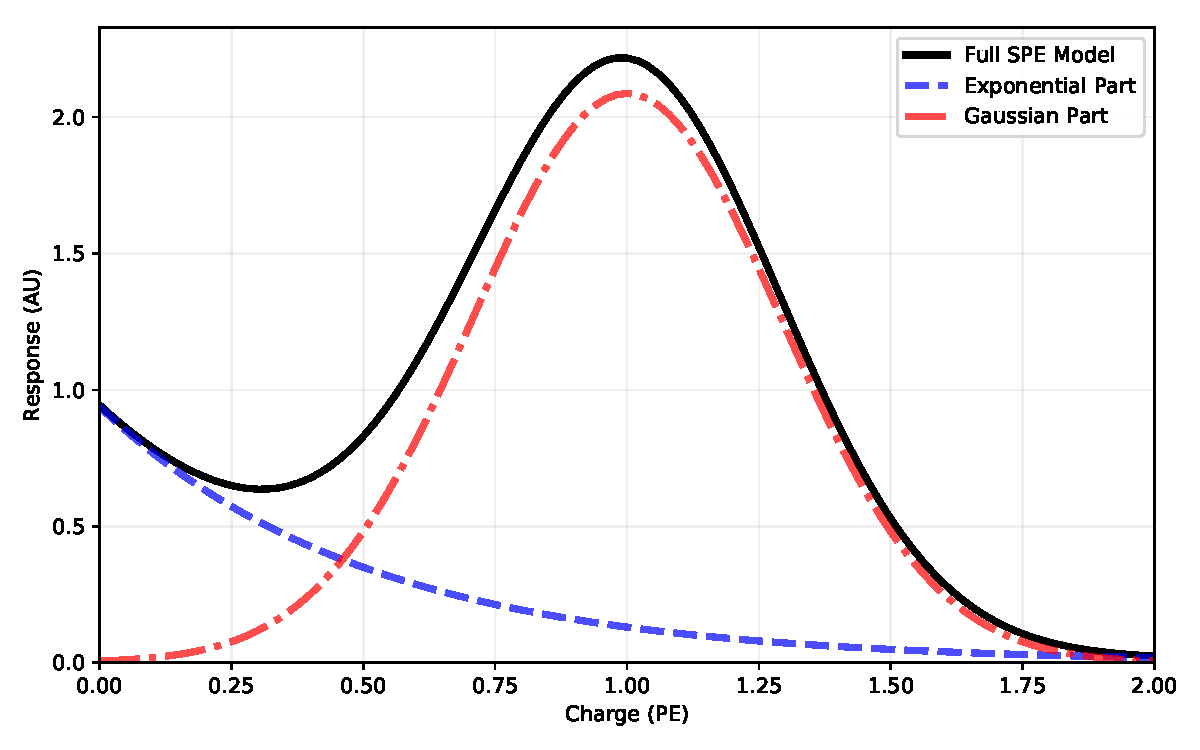
\includegraphics[width=0.7\textwidth]{ta0003.pdf} 
\caption[The SPE template used in IceCube simulation]{The SPE template used in Monte Carlo simulation. The gaussian (red, dash-dot) and exponential (blue, dashed) parts of the full model (black) are shown. The SPE template is used as a sampling distribution for each incident photon in order to determine the observed charge. The SPE template is used for all DOMs.}
\label{fig:ta0003}
\end{figure}

The first module, \emph{PMTResponseSimulator}, simulates the amplification process of the PMT, including the effects of pre-, late-, and afterpulsing.
Each of these three effects is modeled using calibration measurements performed in the lab \cite{IceCube-PMT}.
PMTResponseSimulator also calculates the amount of charge recorded by the DOM from each incident photon reaching the photocathode by sampling from the \emph{single photoelectron} template (\emph{SPE} template).
The SPE template used in simulation generation is calculated from lab measurements of 118 DOMs prior to deployment \cite{TA0003}.
The template, shown in Figure~\ref{fig:ta0003}, is represented by the sum of an exponential and gaussian term and is applied identically to all DOMs.

Prepulses, late pulses, and afterpulses are applied in a recursive process, which every incident hit having a probability of 0.3\%, 3.5\%, and 5.93\% to produce each respectively.
These probabilities were measured in the lab and are used for all DOMs. 

The second module, \emph{DOMLauncher}, handles the local coincidence circuits, simulation of the DOM clock, the discriminator, and digitization.
The triggering system is then applied following the description of Section~\ref{subsec:triggers}.




